\documentclass[a4paper]{article}

\usepackage[english]{babel}
\usepackage[utf8]{inputenc}
\usepackage{fullpage}
\usepackage{amsmath}
\usepackage{graphicx}
\usepackage[colorinlistoftodos]{todonotes}
%\usepackage{hyperref}
\usepackage{amssymb}
\usepackage{subfigure}
\usepackage{url}
\usepackage[pagebackref=true,colorlinks,linkcolor=red,citecolor=green,breaklinks=true,bookmarks=false]{hyperref}
\usepackage{outline} 
\usepackage{pmgraph} \usepackage[normalem]{ulem}
\usepackage{graphicx} \usepackage{verbatim}
\usepackage{indentfirst}
\usepackage{listings}
\usepackage{xcolor}
\lstset{
	numbers=left, 
	numberstyle= \tiny, 
	keywordstyle= \color{ blue!70},
	commentstyle= \color{red!50!green!50!blue!50}, 
	frame=shadowbox, % 阴影效果
	rulesepcolor= \color{ red!20!green!20!blue!20} ,
	escapeinside=``, % 英文分号中可写入中文
	xleftmargin=2em,xrightmargin=2em, aboveskip=1em,
	framexleftmargin=2em
} 
\setlength{\parindent}{2em}
% \usepackage{minted} % need `-shell-escape' argument for local compile

\title{
    \vspace*{1in}
    
\includegraphics[width=2.75in]{figures/zhenglab-logo} \\
    \vspace*{1.2in}
    \textbf{\huge Weekly Work Report}
    \vspace{0.2in}
}

\author{Hongzhi Liu \\
    \vspace*{0.5in} \\
    \textbf{VISION@OUC} \\
    \vspace*{1in}
}

\date{\today}


\begin{document}
\par
\maketitle
\setcounter{page}{0}
\thispagestyle{empty}

\newpage

\section{Research problem}

During this period of week, I spend time studying deep learning courses and working about Faster R-CNN algorithm for off-line test and FGFA algorithm for video object detection method in order to prepare URPC2018. Our team need to train 12 models that includes 11 kinds of image restoration and one image enhancement methods then output txt documents to evaluate algorithm performance with Yolo. Furthermore, I try to solve the error problems in running train code of flow-guided feature aggregation for video object detection.

Because of difficulty in code modification, I have difficulty in adding codes to realize the function which can read test\_list.txt then output a txt which includes information about picture ID, class, confidence and correct bounding box. However, we realize that what should be tested are picture excluding pictures from training sessions. Then, I spend much time deleting items that are not required in test\_list.txt. At last, I should try to train a contest model by using flow guided feature aggregation algorithm. 

\section{Research approach}

In the process of research, I use the method of documentary analysis, comparative analysis and experimental research method. I read the thesis of Fast R-CNN \cite{Girshick2015Fast}, Faster R-CNN algorithm \cite{Ren2015Faster} and flow guided feature aggregation \cite{zhu17fgfa}. I try to unferstand core ideology in paper and learn about concept introduced by author.

Besides, I learn grammatical structure of python on the one hand, and on the other hand, I try to write script files to achieve batch processing commands. By this method, I can have a better understanding of python.

For deep learning, I watch the fifth course videos and write down the issues which I think are much important for further research. And then, I not only have learned the lessons of deep learning, but also put them into coding action. 


\section{Research progress}

During preparation for URPC2018, I receive an image enhancement datasets to train models and test how good the restoration algorithm are with mAP values. I continue to learn about Faster R-CNN algorithm \cite{Ren2015Faster} and relevant theory of flow guided feature aggregation \cite{zhu17fgfa}. Furthermore, I compare the results of 11 image restoration methods that are clahe2, clahe6, hsv, dcp, dcp\_guided, dcp(red), dcp(red)+guided, dcp+clahe, dcp(red)+clahe, ssim and ssim5 as well as 1 enhancement method after test with pictures from 2018URPC. By using the remote server, I try to train contest models with FGFA algorithm and solve the porblem encounted when running a program with help of senior student. I will list details about weekly work in Tab.~\ref{t1} below.

\begin{table}[hb]
	\centering
	\caption{Weekly work progress.}
	\begin{tabular}{c|p{10cm}}
		\hline 
		& Finish training and testing 11 kinds of image restoration methods.\\
		
		& Finish preparing data sets and xml files of 20307 pictures for training the enhancement method. \\
		
		URPC2018 & Finish resizing pictures and modified test\_list file to evaluate performance of models.\\
		
		& Finish comparing mAP value of 12 methods and judge which are better.\\
		
		& Finish solving several error problems when running FGFA algorithm.\\
		\hline
		Deep Learning& Finish learning Sequence Models which is the fifth course of deep learning.\\
		\hline
	\end{tabular}
	\label{t1}
\end{table} 


\section{Progress in this week}

During preparation for URPC2018, I have reordered four image restoration datasets upload to server. Then I spend time checking why output results of mAP value is too low and know the reason finally. After getting the correct result of mAP value of four image restoration methods, we compare them with origin picture to sum up experience. Besides, I modified code to make the output text is in correct method according to the official description. Furthermore, I can  run a FGFA demo and solve the problem in running code.  
\begin{description}
	\item[Step 1] Finish modifying test\_list.txt and delete items that are not required in it in order to choose test pictures for evaluation.
	\item[Step 2] Finish training and testing 11 kinds of image restoration methods.
	\item[Step 3] Finish preparing data sets and xml files of enahnced pictures for training the method.
	\item[Step 4] Finish learning Sequence Models which is the fifth lesson.\label{t2}
\end{description}

\subsection{Data Sets}

In this week, our team received an enhanced method which includes six data sets more than twenty thousand pictures as shown in Fig.~\ref{p1}. We train the contest model with the these datasets. Besides, I reordered B3, B4, B5, B6, green and blue pictures to train and test. Fig.~\ref{p1}\subref{p1a} is the picture restored by B3 method, Fig.~\ref{p1}\subref{p1b} is the picture restored by B4 method. Fig.~\ref{p1}\subref{p1c} is the picture restored by B5 method. Fig.~\ref{p1}\subref{p1d} is the picture restored by B6 method. Fig.~\ref{p1}\subref{p1e} is the picture restored by green method. Fig.~\ref{p1}\subref{p1f} is the picture restored by blue method. And we use Algorithm~\ref{g1} to modified frame name in xml files to VOC format.
\begin{figure}
	\centering 
	\subfigure[]{ 
		\label{p1a} %% label for first subfigure 
		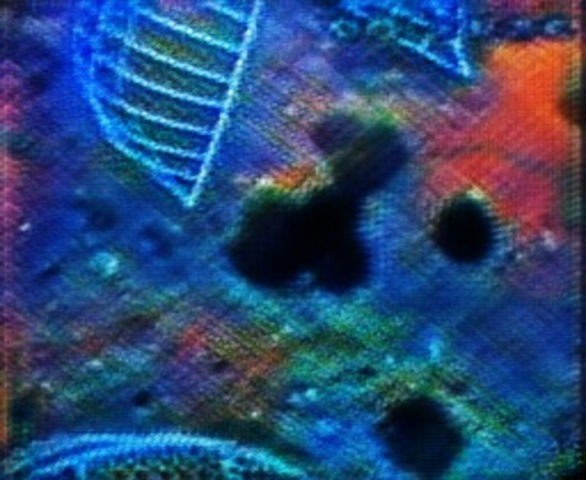
\includegraphics[width=7cm]{figures/1.jpg} 
	} 
	\subfigure[]{ 
		\label{p1b} %% label for second subfigure 
		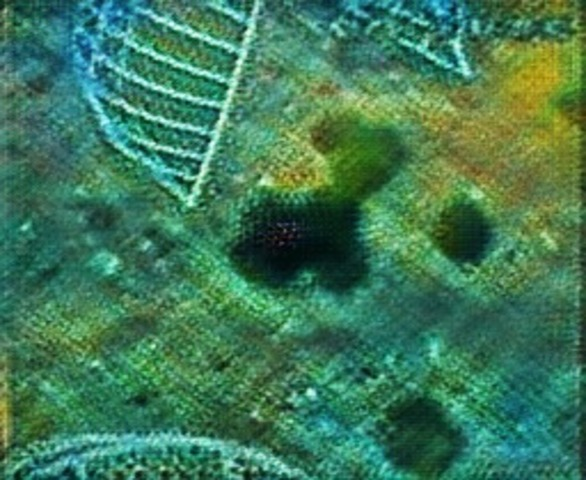
\includegraphics[width=7cm]{figures/2.jpg} 
	} 
	\subfigure[]{ 
		\label{p1c} %% label for second subfigure 
		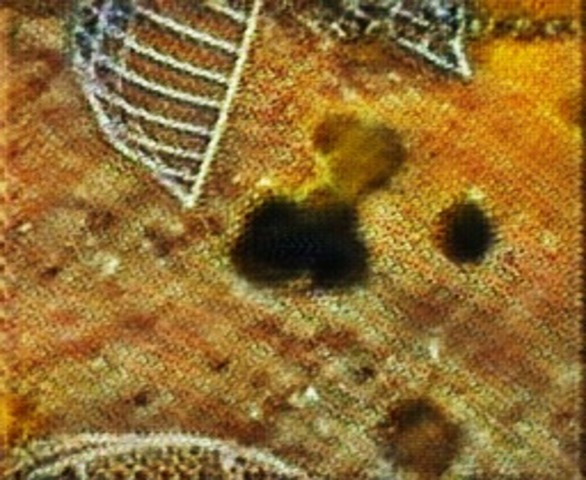
\includegraphics[width=7cm]{figures/3.jpg} 
	} 
	\subfigure[]{ 
		\label{p1d} %% label for second subfigure 
		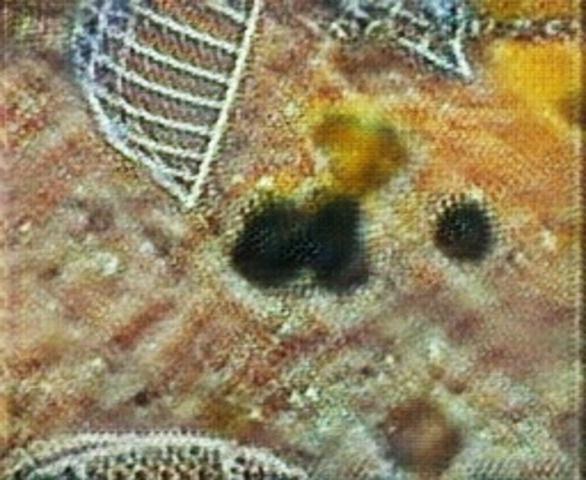
\includegraphics[width=7cm]{figures/4.jpg} 
	} 
	\subfigure[]{ 
		\label{p1e} %% label for second subfigure 
		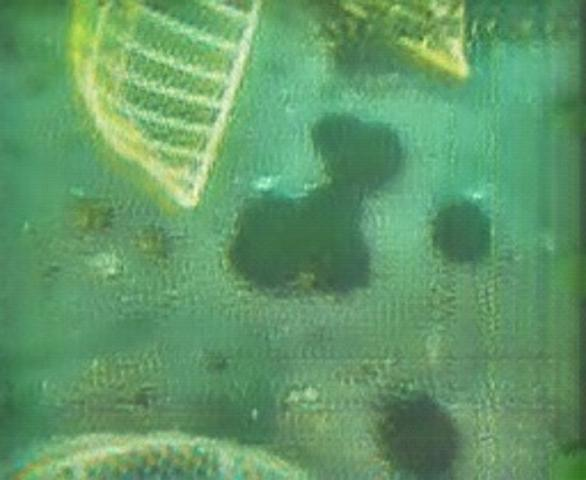
\includegraphics[width=7cm]{figures/5.jpg} 
	} 
	\subfigure[]{ 
		\label{p1f} %% label for second subfigure 
		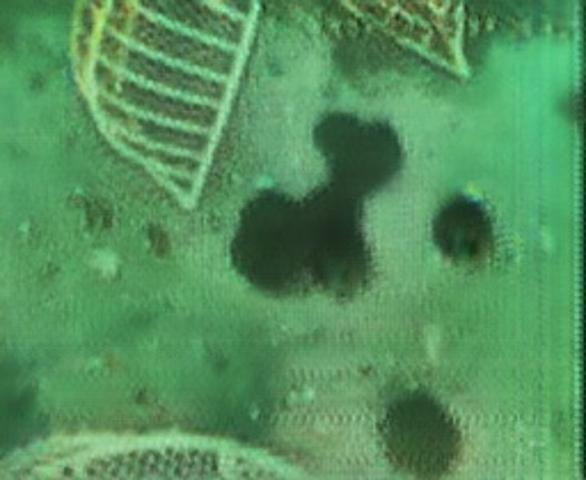
\includegraphics[width=7cm]{figures/6.jpg} 
	} 
	\caption{The same picture is enhanced by six kinds of image enhancement method.} 
	\label{p1} %% label for entire figure 
\end{figure}

\begin{figure}
	\centering 
	\subfigure[]{ 
		\label{p2a} %% label for first subfigure 
		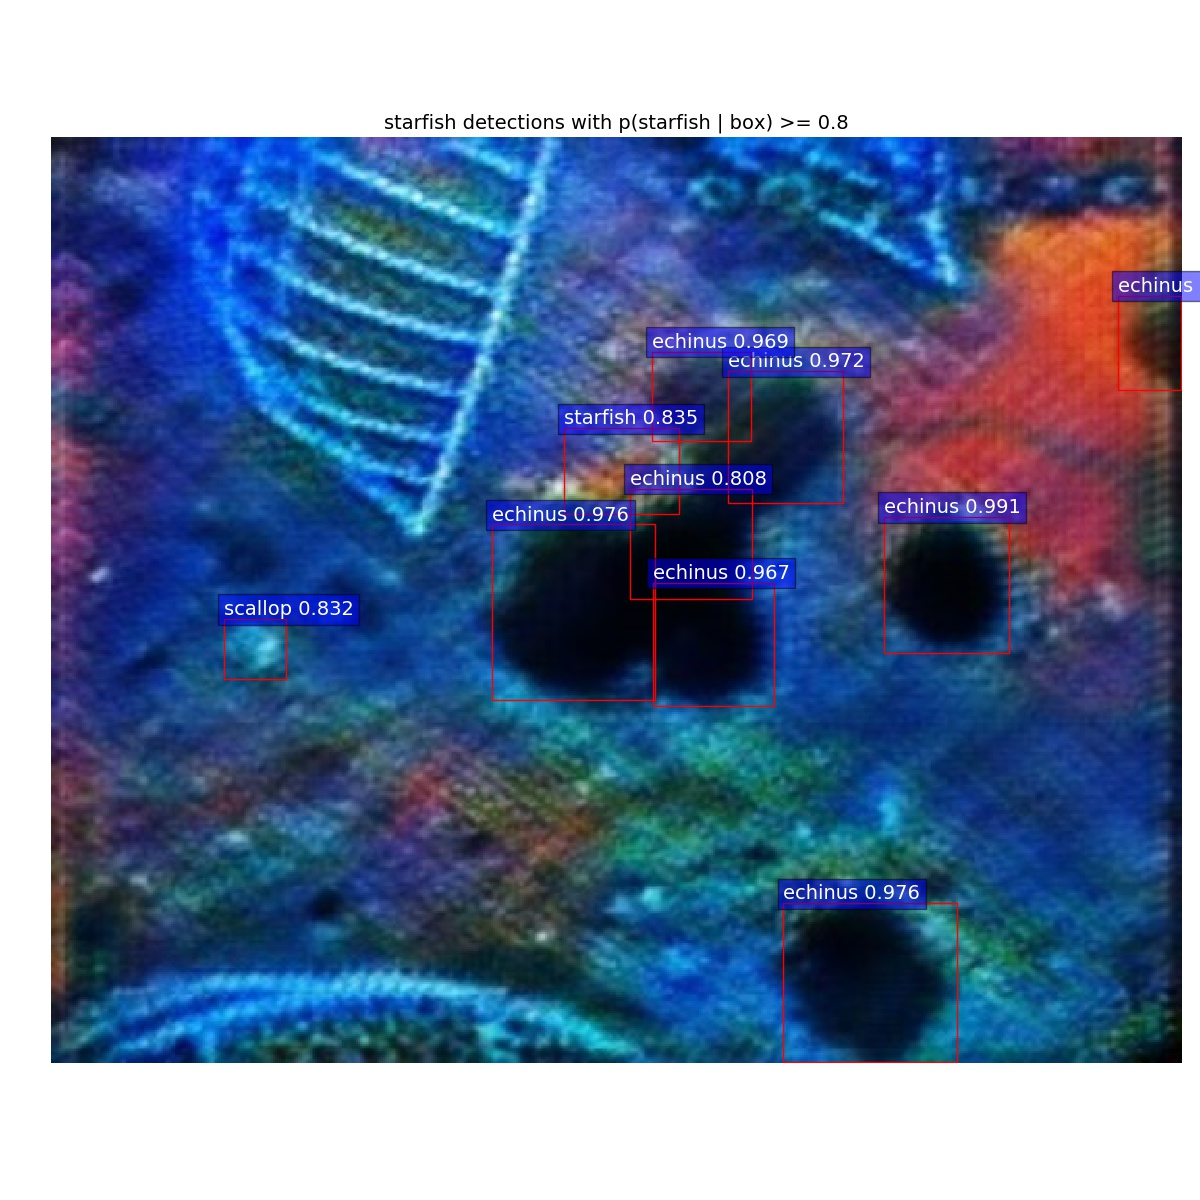
\includegraphics[width=7cm]{figures/8.jpg} 
	} 
	\subfigure[]{ 
		\label{p2b} %% label for second subfigure 
		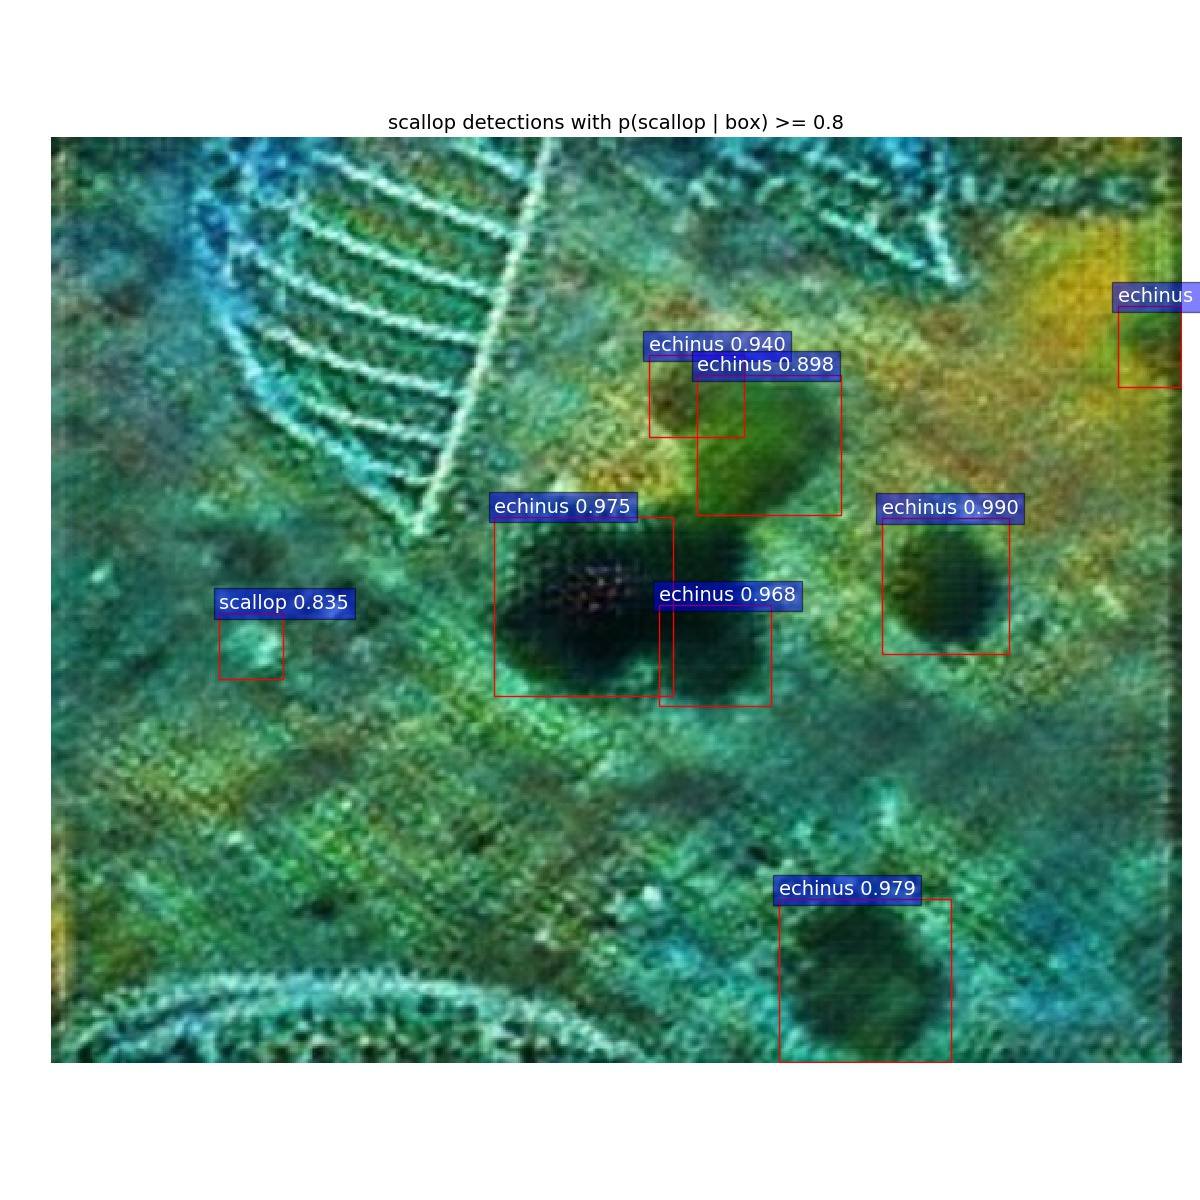
\includegraphics[width=7cm]{figures/9.jpg} 
	} 
	\subfigure[]{ 
		\label{p2c} %% label for second subfigure 
		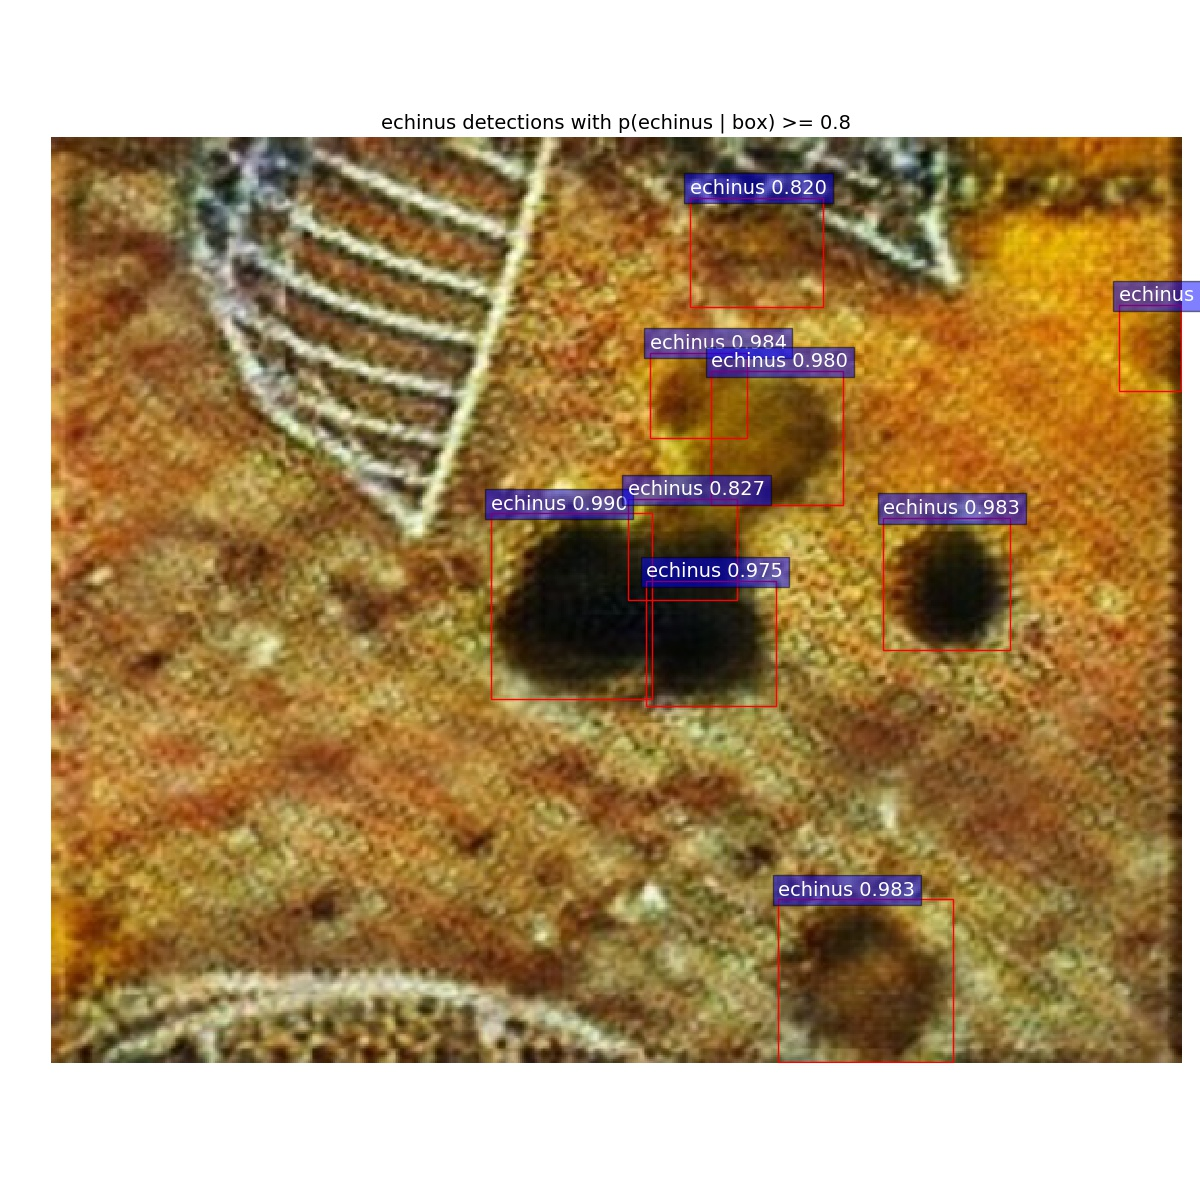
\includegraphics[width=7cm]{figures/10.jpg} 
	} 
	\subfigure[]{ 
		\label{p2d} %% label for second subfigure 
		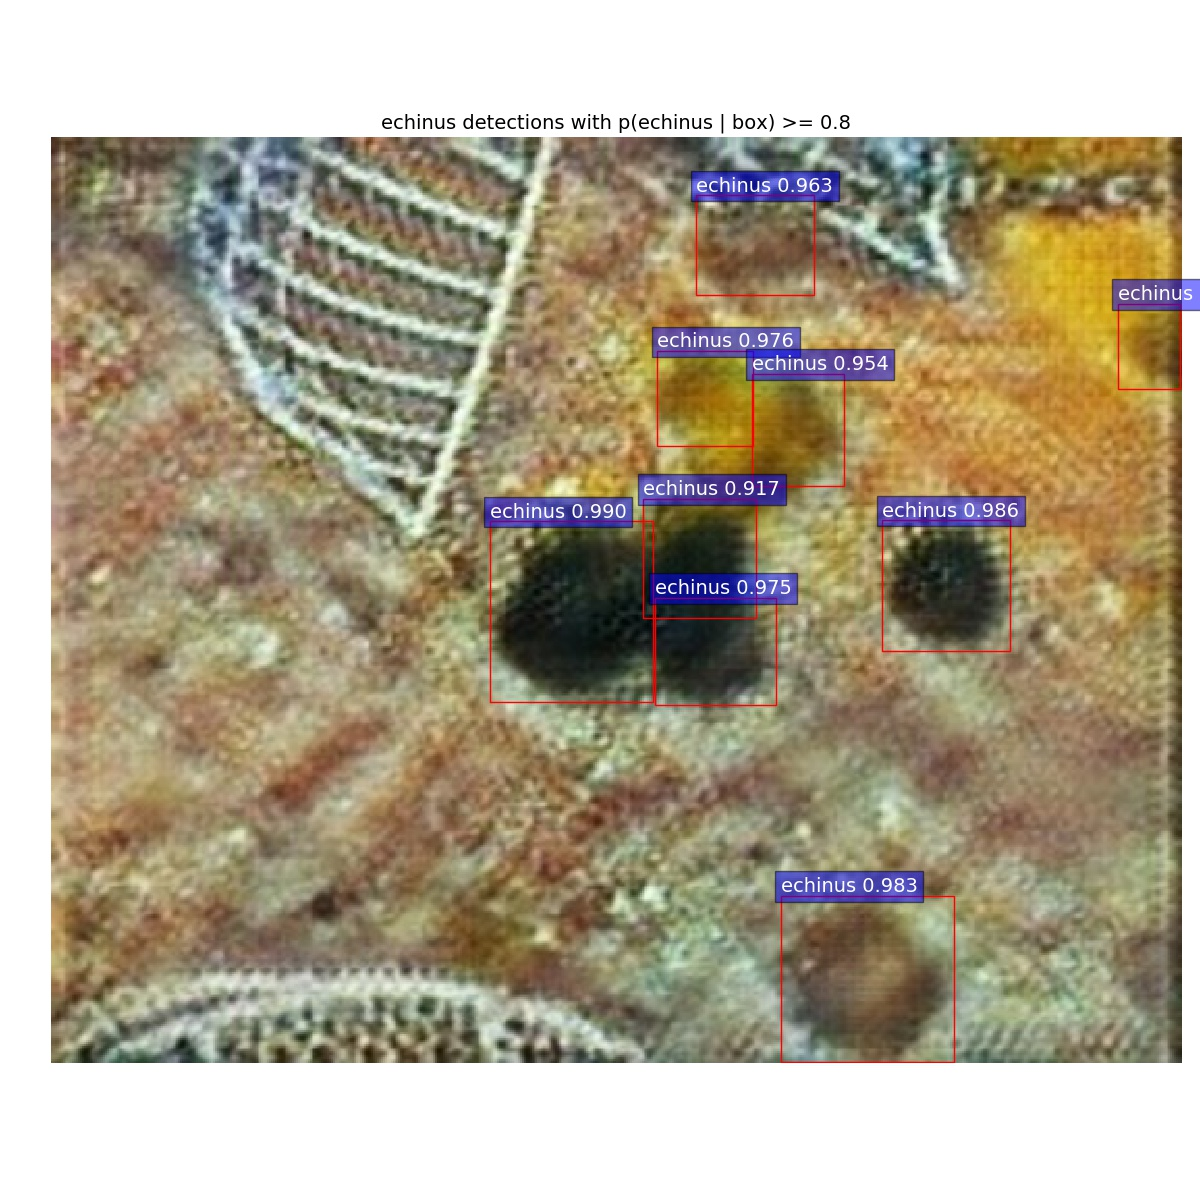
\includegraphics[width=7cm]{figures/11.jpg} 
	} 
	\subfigure[]{ 
		\label{p2e} %% label for second subfigure 
		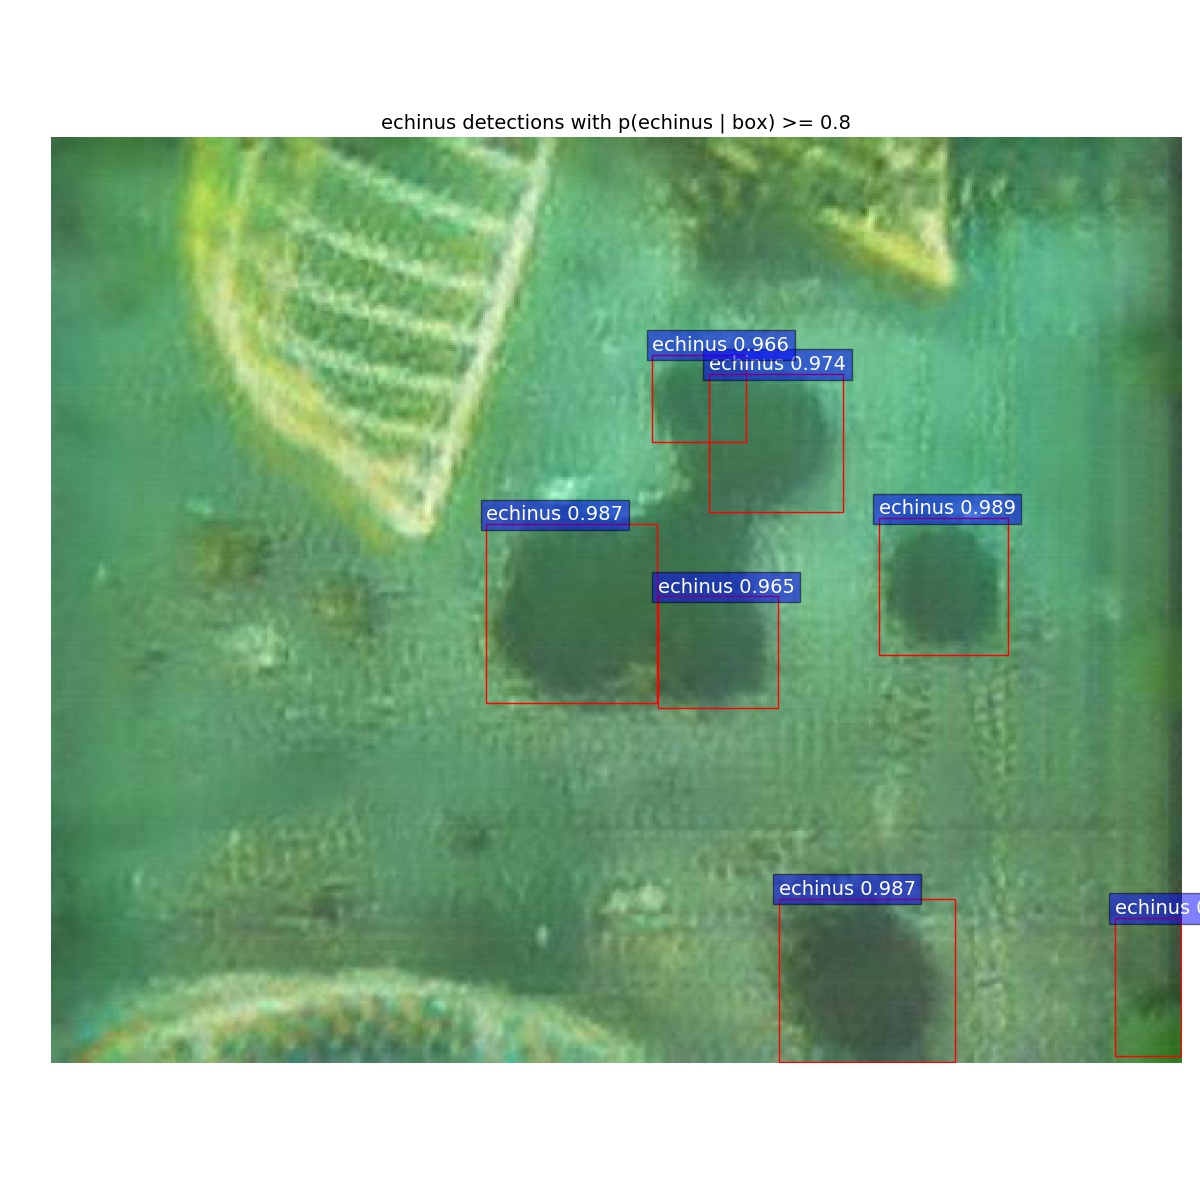
\includegraphics[width=7cm]{figures/12.jpg} 
	} 
	\subfigure[]{ 
		\label{p2f} %% label for second subfigure 
		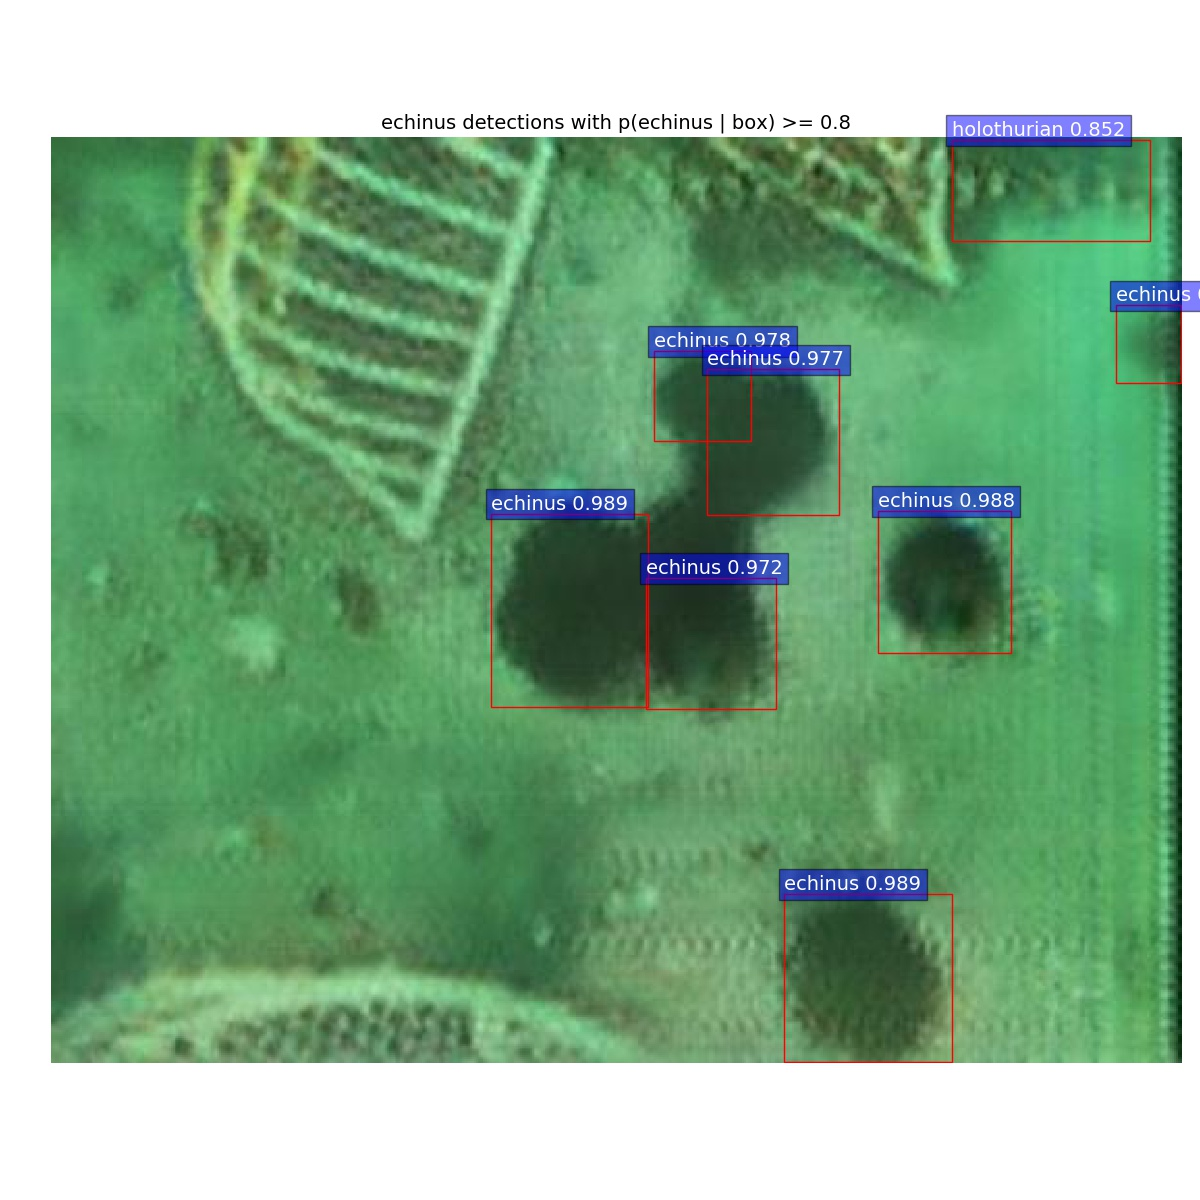
\includegraphics[width=7cm]{figures/13.jpg} 
	} 
	\caption{The bounding boxes in the same picture which is enhanced by six kinds of image enhancement method.} 
	\label{p2} %% label for entire figure 
\end{figure}

\lstset{language=python}
\begin{lstlisting}
#coding=utf-8
import os
import os.path
import xml.dom.minidom
path="./enhance0815"
files=os.listdir(path)
s=[]
for xmlFile in files:
portion = os.path.splitext(xmlFile)
if not os.path.isdir(xmlFile):
dom=xml.dom.minidom.parse(os.path.join(path,xmlFile))
root=dom.documentElement
name=root.getElementsByTagName('frame')
for i in range(len(name)):
print(xmlFile)
if portion[1] ==".xml":           
newname = portion[0]+".jpg"
print(newname)
name[i].firstChild.data=newname
print (name[i].firstChild.data)
with open(os.path.join(path,xmlFile),'w',encoding='UTF-8') as fh:
dom.writexml(fh)
print('修改filename OK!')
\end{lstlisting}\label{g1}

\subsection{Test a Contest Model}

Accodting to the six data sets of image enhancement method, we train the model and get the results of it can be seen in Fig.~\ref{p3}. Each picture with a bounding box in Fig.~\ref{p2}, corresponding to the picture mentioned in Fig.~\ref{p1} above.

During the mobel testing, our team spend time modifying test\_list.txt which includes 581 items. Then we use Algorithm~\ref{g2} to run a train process to get the result of mAP value.

\begin{figure}
	\begin{center}
		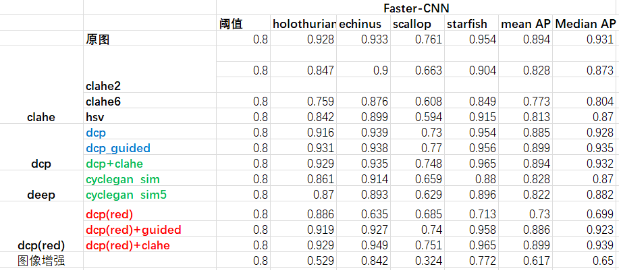
\includegraphics[scale=0.6]{figures/7.png}
	\end{center}
	\caption{Output results of several methods.}
	\label{p3}
\end{figure}

\lstset{language=python}
\begin{lstlisting}
def demo(sess, net, image_name):
# Load the demo image
print('demoDemo for data/demo/{}{}'.format(im_name[0], '.jpg'))
print('demoDemo for data/demo/{}{}'.format(im_name[1], '.jpg'))
print('\n')

all_name = image_name+'.jpg'
im_file = os.path.join(cfg.DATA_DIR, 'demo', all_name)
im = cv2.imread(im_file)

fr = open('/home/henry/Files/tf-faster-rcnn-contest/data/
VOCdevkit2007/test_list.txt', 'r')
for im_name in fr:
im_name = im_name.strip()
im_name = im_name.split(' ')
print('~~~~~~~~~~~~~~~~~~~~~~~~~~~~~~~~~~~')
print('mainDemo for data/demo/{}{}'.format(im_name[0],'.jpg'))
print('mainDemo for data/demo/{}{}'.format(im_name[1],'.jpg'))
print('\n')
demo(sess, net, im_name[0])
\end{lstlisting}\label{g2}

\subsection{Training of FGFA Algorithm}

There are some difficulties running the demo for us because of little issue reference in the github and blogs. So senior student and I try our best to solve the problems as~\ref{g3}.

\lstset{language=python}
\begin{lstlisting}
In file included from src/operator/tensor/././sort_op.h:85:0,
from src/operator/tensor/./indexing_op.h:24,
from src/operator/tensor/indexing_op.cu:8:
src/operator/tensor/./././sort_op-inl.cuh:10:44: 
fatal error: cub/device/device_radix_sort.cuh: No such file or directory
#include <cub/device/device_radix_sort.cuh>
^
compilation terminated.
make: *** [build/src/operator/tensor/indexing_op_gpu.o] Error 1
\end{lstlisting}\label{g3}

We find the error about cub and then modify some codes to compile. Finally, we get over these difficulty but still have some to deal with. 


\section{Plan}

\begin{tabular}{rl}
	\textbf{Objective:} & Finish open ROV equipment debugging and FGFA training. \\
	\textbf{Deadline:} & 2018.08.25
\end{tabular}

\begin{description}
	\item[\normalfont 2018.08.13---2018.08.19] Finish sequence models courses.
	\item[\normalfont 2018.08.20---2018.08.26] Finish evaluation of Faster RCNN.
	\item[\normalfont 2018.08.27---2018.09.02] Finish preparation of 2018URPC.
\end{description}



% If you don't cite any references, please comment the following two lines
\bibliographystyle{ieee}
\bibliography{ref.bib}

\end{document}